% This is text associated with the open remixable textbook "Open Electromagnetics"
% See immediately below for author, date
% <License info goes here (boilerplate, not read by project compiler)>

%ORB TITLE Electromagnetic Spectrum  
%ORB AUTHOR 0        # S.W. Ellingson, Virginia Tech (ellingson@vt.edu)
%ORB DATE   20180731 # yyyymmdd
%ORB ABSTRACT Introduction to planar, cylindrical, and spherical waves

\label{m0075_Electromagnetic_Spectrum} % <-- Must match name of this file and module directory name.  Don't mess with this!

Electromagnetic fields exist at frequencies from DC (0~Hz) to at least $10^{20}$~Hz -- that's at least 20 orders of magnitude!

At DC, electromagnetics consists of two distinct disciplines: \emph{electrostatics}, concerned with electric fields; and \emph{magnetostatics}, concerned with magnetic fields.

At higher frequencies, electric and magnetic fields interact to form propagating waves.
Waves having frequencies within certain ranges are given names based on how they manifest as physical phenomena. 
These names are (in order of increasing frequency):
\emph{radio},
\index{radio (frequency)}
\emph{infrared} (IR),
\index{infrared}
\emph{optical} (also known as ``light''),
\index{optical (frequency)}
\emph{ultraviolet} (UV),
\index{ultraviolet}
\emph{X-rays}, and
\index{X-ray}
\emph{gamma rays} ($\gamma$-rays).
\index{gamma ray}
See Table~\ref{m0075_tEMS} and Figure~\ref{m0075_fEMS} for frequency ranges and associated wavelengths.

%ORB HIGHLIGHT
\begin{mdframed}[backgroundcolor=yellow!20,nobreak=true] 
The term \emph{electromagnetic spectrum} 
\index{spectrum}
\index{electromagnetic spectrum|see{spectrum}}
refers to the various forms of electromagnetic phenomena that exist over the continuum of frequencies.
\end{mdframed}

\begin{table*}[t]
\begin{center}
\begin{tabular}{lcc}
Regime & Frequency Range & Wavelength Range \\
\hline
$\gamma$-Ray & $>3\times 10^{19}$~Hz & $<0.01$~nm   \\
X-Ray & $3\times 10^{16}$~Hz -- $3\times 10^{19}$~Hz & 10--0.01~nm  \\
Ultraviolet (UV) & $2.5\times 10^{15}$ -- $3\times 10^{16}$~Hz & 120--10~nm  \\
Optical & $4.3\times 10^{14}$ -- $2.5\times 10^{15}$~Hz & 700--120~nm  \\
Infrared (IR) & 300~GHz -- $4.3\times 10^{14}$~Hz & 1~mm -- 700~nm  \\
Radio & 3~kHz -- 300~GHz & 100~km -- 1~mm  \\
\end{tabular}
\end{center}
\caption{The electromagnetic spectrum.  Note that the indicated ranges are arbitrary but consistent with common usage.}
\label{m0075_tEMS}
%\label{cIntro_fEMS}
\end{table*}

The speed (properly known as ``phase velocity'') 
\index{phase velocity}
at which electromagnetic fields propagate in free space is given the symbol $c$, and has the value $\cong 3.00 \times 10^8$~m/s. 
% https://en.wikipedia.org/wiki/Speed_of_light
This value is often referred to as the ``speed of light.''
\index{speed of light}
While it is certainly the speed of light in free space, it is also speed of \emph{any} electromagnetic wave in free space.
Given frequency $f$, wavelength 
\index{wavelength}
is given by the expression
$$
\lambda=\frac{c}{f}~~\mbox{in free space}
$$
Table~\ref{m0075_tEMS} shows the free space wavelengths associated with each of the regions of the electromagnetic spectrum.

This book presents a version of electromagnetic theory that is based on classical physics.
This approach works well for most practical problems. 
However, at very high frequencies, wavelengths become small enough that quantum mechanical effects may be important.
This is usually the case in the X-ray band and above.
In some applications, these effects become important at frequencies as low as the optical, IR, or radio bands. (A prime example is the \emph{photoelectric effect}; 
\index{photoelectric effect}
see ``Additional References'' below.)
Thus, caution is required when applying the classical version of electromagnetic theory presented here, especially at these higher frequencies.

%ORB HIGHLIGHT
\begin{mdframed}[backgroundcolor=yellow!20,nobreak=true] 
Theory presented in this book is applicable to DC, radio, IR, and optical waves, and to a lesser extent to UV waves, X-rays, and $\gamma$-rays.
Certain phenomena in these frequency ranges -- in particular quantum mechanical effects -- are not addressed in this book.
\end{mdframed}

The radio portion of the electromagnetic spectrum alone spans 12 orders of magnitude in frequency (and wavelength), and so, not surprisingly, exhibits a broad range of phenomena.  This is shown in Figure~\ref{m0075_fEMS}. For this reason, the radio spectrum is further subdivided into bands as shown in Table~\ref{m0075_tRFS}.  Also shown in Table~\ref{m0075_tRFS} are commonly-used band identification acronyms and some typical applications.  
%
\begin{figure}
\begin{center}
\pdftooltip{{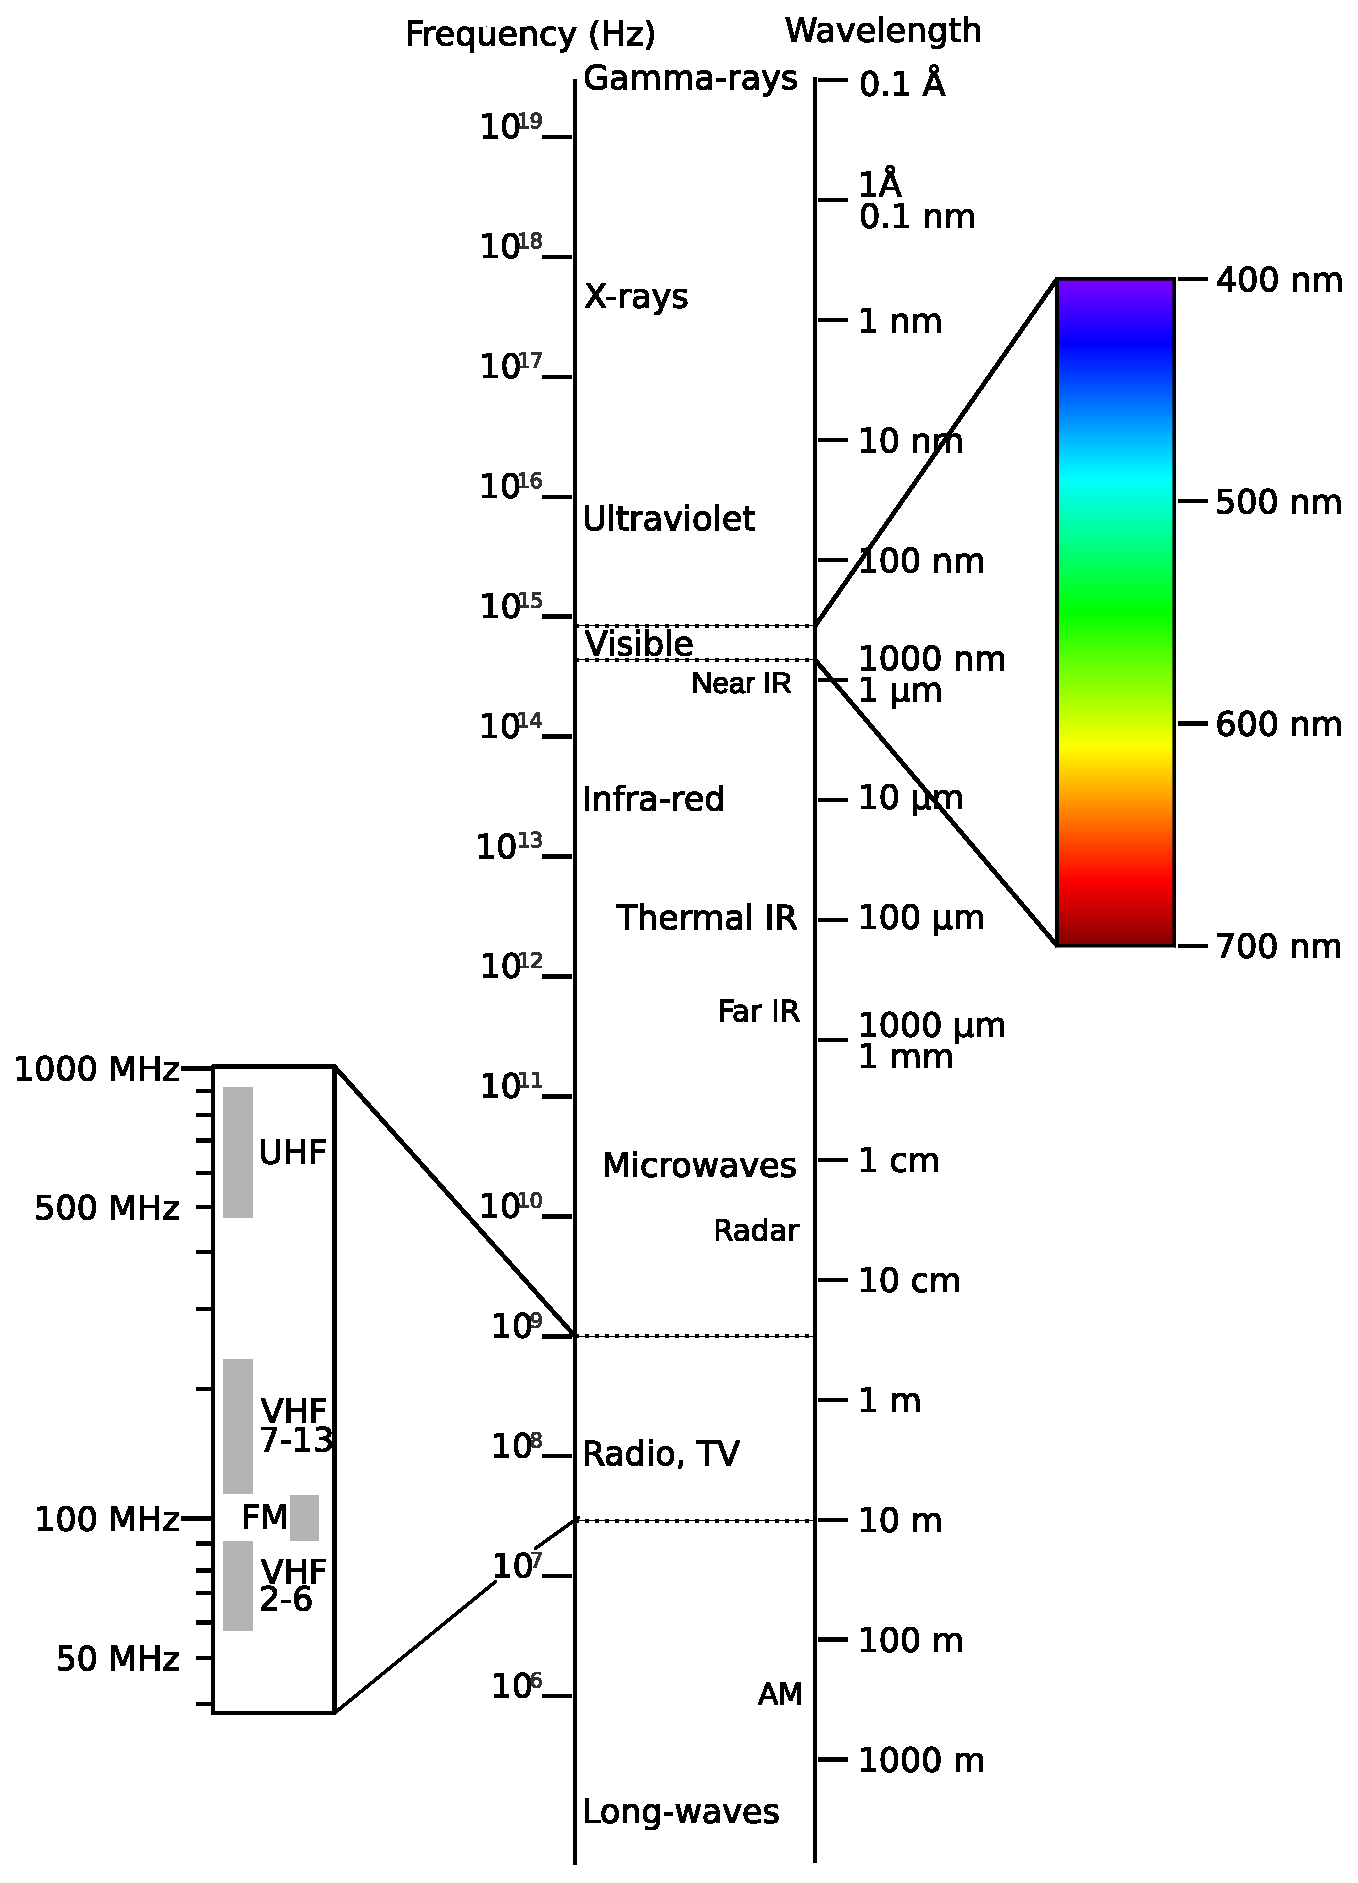
\includegraphics[width=\columnwidth]{modules/m0075_fEMS.eps}}}{A graphical depiction of the range of the electromagnetic spectrum in terms of frequency (10 raised to 6 to 10 raised to 19 Hz) and wavelength (1000 m to 0.01 nm). Shown as a tall rectangle, highlighted spectra are the radio spectrum (50 MHz to 1000 MHz from bottom to top) and the wavelengths in the optical band (700 nm to 400 nm from bottom to top).}
\end{center} 
%\vspace{2in}
% https://commons.wikimedia.org/wiki/File:Electromagnetic-Spectrum.svg
\centerline{\scriptsize 
\copyright~\hyperref[m0075_fEMS_Credit]{V.\ Blacus} 
\href{https://creativecommons.org/licenses/by-sa/3.0/}{CC BY-SA 3.0} 
} 
\caption{
\label{m0075_fEMS}
Electromagnetic Spectrum.
}
\end{figure}
%
\begin{table*}[t]
\begin{center}
\begin{tabular}{lccl}
Band & Frequencies & Wavelengths & Typical Applications \\
\hline
EHF & 30-300~GHz & 10--1~mm & 60~GHz WLAN, Point-to-point data links \\
SHF & 3--30~GHz & 10--1~cm & Terrestrial \& Satellite data links, Radar \\ 
UHF & 300--3000~MHz & 1--0.1~m & TV broadcasting, Cellular, WLAN \\
VHF & 30--300~MHz & 10--1~m & FM \& TV broadcasting, LMR \\ 
HF & 3--30~MHz & 100--10~m & Global terrestrial comm., CB Radio \\
MF & 300--3000~kHz & 1000--100~m & AM broadcasting \\
LF & 30--300~kHz & 10--1~km & Navigation, RFID \\
VLF & 3--30~kHz & 100--10~km & Navigation \\
\end{tabular}
\end{center}
\caption{The radio portion of the electromagnetic spectrum, according to a common scheme for naming ranges of radio frequencies. WLAN: Wireless local area network, LMR: Land mobile radio, RFID: Radio frequency identification.}
%\label{cIntro_fRFS}
\label{m0075_tRFS}
\end{table*}

Similarly, the optical band is partitioned into the familiar ``rainbow'' of red through violet, as shown in Figure~\ref{m0075_fEMS} and Table~\ref{m0075_tOptical}. Other portions of the spectrum are sometimes similarly subdivided in certain applications.
%
%\begin{table*}[t]
\begin{table}
%\vspace{3in}
\begin{center}
\begin{tabular}{lcc}
Band & Frequencies & Wavelengths \\
\hline
Violet & 668--789~THz & 450--380~nm  \\
Blue   & 606--668~THz & 495--450~nm  \\
Green  & 526--606~THz & 570--495~nm  \\ 
Yellow & 508--526~THz & 590--570~nm  \\
Orange & 484--508~THz & 620--590~nm  \\
Red    & 400--484~THz & 750--620~nm  \\
\end{tabular}
\end{center}
\caption{The optical portion of the electromagnetic spectrum.}
% https://en.wikipedia.org/wiki/Visible_spectrum 
\label{m0075_tOptical}
%\end{table*}
\end{table}

%%% https://commons.wikimedia.org/wiki/File:Atmospheric_electromagnetic_opacity.svg

{\bf Additional Reading:}
\begin{itemize}
\item ``\href{https://en.wikipedia.org/wiki/Electromagnetic_spectrum}{Electromagnetic spectrum}'' on Wikipedia.
\item ``\href{https://en.wikipedia.org/wiki/Photoelectric_effect}{Photoelectric effect}'' on Wikipedia.
\end{itemize}

